%!TEX encoding = UTF-8 Unicode
%!TEX program = xelatex

\documentclass[bachelor]{ustcthesis}
% bachelor|master|doctor
\usepackage{ustcextra}
\usepackage{color}
\usepackage{ulem}
\graphicspath{{figures/}}
\bibliographystyle{ustcauthoryear}
% \bibliographystyle{ustcnumerical}

\renewpagestyle{front}[\zihao{-5}]{
    \sethead{}{软件工程即时通讯系统概要设计}{}
    \setfoot{}{\thepage}{}
    \headrule
}
\renewpagestyle{main}[\zihao{-5}]{
    \sethead{}{软件工程即时通讯系统概要设计}{}
    \setfoot{}{\thepage}{}
    \headrule
}
\newcommand{\HRule}{\rule{\linewidth}{0.5mm}}
\newcommand{\tabincell}[2]{\begin{tabular}{@{}#1@{}}#2\end{tabular}}

\begin{document}



\begin{titlepage}
\begin{center}
~\\[5cm]
\HRule \\[0.4cm]
{\huge \bfseries 软件工程即时通讯系统\\概要设计}\\[0.4cm]
\HRule \\[1.5cm]

\begin{tabular}{ccc}
  & 人员 & 日期 \\ 
拟制 & 王嵩超\ 罗炳琨\ 龚正 & 2018-05-18 \\ 
评审人 & 罗炳琨 • & 2018-05-19 \\ 
批准 & 罗炳琨 & 2018-05-20 \\ 
签发 & 王嵩超 & 2018-05-20 \\ 
\end{tabular} 

\end{center}
\end{titlepage}



\frontmatter
\begin{abstract}
本文是软件工程13组的需求规格说明书,其模板修改自于中国科学技术大学本硕博毕业论文 \LaTeX{} 模板示例文件,该模板由
zepinglee和seisman创建,遵循中国科学技术大学的论文写作规范,适用于撰写学士、硕士和博士学位论文。

\keywords{软件工程\zhspace{} 中国科学技术大学\zhspace{} 学位论文\zhspace{} \LaTeX{}~通用模板\zhspace{} 学士\zhspace{}
硕士\zhspace{} 博士\zhspace{} 示例文档\zhspace{} 模板说明文档}

% \begin{table}[htbp]
% \centering
% \caption{缩略词清单} \label{tab:abbr}
% \begin{tabular}{|c|c|c|}
%     \hline
%     缩略语 & 英文全名 & 中文解释 \\
%     \hline
%     c & d & e\\
%     \hline
% \end{tabular}
% \end{table}

\end{abstract}

\tableofcontents
\listoffigures
\listoftables
% \listofalgorithms  % 算法索引,如不需要,可直接注释掉本行
% \begin{notation}

%\centering
%XX 软件需求规格说明书

%关键词:能够体现文档描述内容主要方面的词汇。
 
%摘要:


\centering
\begin{tabular}{rl}
$\ln x$ & natural logarithm $\log_ex$ \\
$\log x$ & common logarithm $\log_{10}x$ \\
$x\ \mathrm{mod}\ y$ & remainder \\
\end{tabular}

\end{notation}


\mainmatter
\chapter{简介}
\section{目的}
%This section should state the purpose of the document. It could also specify the intended audience. Identify the product whose software requirements are specified in this document.

%这部分要描述文档的目的。应该指明读者。说明本需求文档描述了哪个产品的软件需求。

本文档为软件工程课程实验二即时通讯系统的需求说明文档。编写该本文档的主要目的是对即时通讯系统的软件需求进行说明,为该系统的详细设计、开发工作提供依据,为项目设计人员、开发人员、使用人员和其他相关人员对系统实现的功能达成统一的认识提供一个明确的书面说明。

本文档的主要读者为项目设计人员,软件开发、测试人员,指导人员,以及目标用户等。

\section{范围}
% This section should address areas which this document includes and that are specifically excludes. 

% 本节应描述文档所包括和不包括的内容。
本文档包括了以需求为中心的相关要求,包括产品所处在的运行环境,所有的功能需求,性能需求,质量特性。
\linebreak
本文档不包括产品的开发、实现等细节内容。

\chapter{总体概述}

%Describes the general elements that may affect the product and the requirements on the product. It includes the following four parts. Note that this section should not describe the specific requirements, instead, it makes the specific requirements to be described more understandable.

%本节描述影响产品和产品需求的一般因素。由以下4个部分构成。 有一点需说明的是本节不描述具体的需求,只是使那些将要描述的具体需求更易于理解。
\section{软件概述}
\subsection{项目介绍}
%Describe the context and origin of the project being specified in this SRS. For example, state whether this project is a follow-on member of a project family, a replacement for certain existing systems, or a new, self-contained project.

%描述本软件需求所描述的项目的背景。例如:本项目是一系列版本中的一个,或者是替代某个已经存在的系统,还是一个新的独立的项目。

本项目要开发的软件为一个独立的即时通讯系统,为软件工程课程实验二的选题之一。

\subsection{产品环境介绍}
%Describes the whole environment that is composed of this software and other products / projects.
%\begin{itemize}
%\item If this software is independent or fully self-contained, state it here.
%\begin{itemize}
%\item describe the function of each component of that larger system/project, and identify the interfaces.
%\item determine the main external interfaces of this software.( Note: Do not describe the interfaces in detail; the detailed description will be provided in other part of the SRS document.)
%\item describe related hardware of the product and peripheral equipment.( Note: This is only  a general description, not in detail.)
%\end{itemize}
%\end{itemize}

%It is very helpful to describe the main components, interconnection and external interfaces of the larger system/project by Block Diagram. This part should not provide a detailed design solution, or detailed design constraint for the solution (the detailed design constraint will be described in the section of specific requirement). This section is the basis of the design constraints.

%描述的是本产品与其它产品或项目所组成的整体环境。

%1.如果本产品是独立的并完全自我包含,在此说明这一点。

%2.如果SRS定义的产品是更大的系统或项目的组件(此种情形经常发生),那么应:

%	A. 描述此大系统或项目每个组件的功能,并且标识接口。
%
%	B.  确定本软件产品主要外部接口。( 注意:在此部分并不进行这些接口的详细描述;对这些接口的详细描述在SRS的其它 部分提供。)
%    
%    C. 描述相关产品硬件和所使用的外部设备。(  注意:  这只是概述性描述。)
%
%通过方块图来描述大系统或项目的主要组件,互连性以及外部接口将是非常有帮助的。本部分不应提出一个具体的设计解决方案或对解决方案的具体设计约束(具体设计约束将在具体需求章节中描述)。本部分内容是产生设计约束的基础。

本系统最终产品将分为服务端和客户端两大组件。
服务端运行于linux或windows平台上,为客户端提供服务。
客户端运行于linux,windows,android,ios等平台上,为用户提供操作接口。

\section{软件功能}
%Summarizes the major functions that must be implemented through the software, and the functions to be implemented through user operation. Details will be provided in the Specific Requirement, so only a summary (such as a directory list) is needed here. The functions should be organized to make them understandable to the readers, and be appropriate for subsequent design and tests. Diagrams like top-level data flow diagram or object class diagram are recommended to illustrate the relationships among the major requirement groups 
%
%Sometimes, this section can directly refer to the superior specification of the software that allocate the specific requirements to this software ( if existed ).
%The specific requirements should not be described in this section. But this section is the basis of the specific requirements.
%
%概述软件的必须实现的和通过用户操作实现的主要功能。这里只需要进行简要描述(例如目录列表),详细描述在详细需求部分描述。对需求功能进行组织,以便于读者理解,并能指导后续的设计和测试。可以用图表来表示主要需求群组之间的关系,例如:高层的数据流图,面向对象的分析等。
%
%有时此部分所要求的功能概述可以从分配具体功能给此软件产品的更高层规格(如果存在的话)直接引用。
%
%本节不应描述具体需求。但本节内容是具体需求章节的基础。
\begin{itemize}
\item 一对一即时通讯
\item 群聊
\item 语音通话
\item 视频通话
\item 用户配对
\item 表情包管理
\end{itemize}

\section{用户特征}
%List down the basic required characteristics of the user or operator of the system. E.g. the experience, Skill level, required role etc., 
%This part should not describe the specific requirements, instead, it provides the basis for the specific requirements.
%
%列出对用户或系统操作者的要求,如:经验,能力,角色等。
%
%本节不应描述具体需求。但本节内容是具体需求章节的基础。

本系统分为服务端和客户端两大组件。

服务端的主要使用者为有搭建即时通讯系统需求的用户,要求具备一定的计算机知识和运维经验。

客户端的主要使用者为有即时通讯需求的用户,用户无需具备特殊的专业知识,但要求具有一定的计算机使用知识。

\section{假设和依赖关系}
List any assumed factors (as opposed to known facts) that could affect the requirements stated in the SRS. These could include third party or commercial components that you plan to use, issues around the development or operating environment, or constraints. The project could be affected if these assumptions are incorrect, are not shared, or change. Also identify any dependencies the project has on external factors, such as software components that you intend to reuse from another project, unless they are already documented elsewhere (for example, in the vision and scope document or the project plan). 

列出可能影响SRS中需求的所有的假设因素(与已知事实相对而言),包括准备使用的第三方或商业组件,操作和开发环境的问题约束等。如果上述假设不正确、没有被告知或者改变了都将对项目产生影响。列出项目对外部条件的依赖,例如重用其他项目的模块等。如果在其他文档(例如项目计划或范围文档等)里已经描述了,在这里可以不用描述。

\chapter{总体设计}
\section{软件描述}
%系统包括前台和后台两个部分。

%前台主要功能是:

%后台主要功能是:
系统包括客户端和服务端两个部分。

客户端为用户提供图形界面,用户可以在客户端上登陆账号,搜索添加好友,和好友聊天,参与群聊,发送语音视频消息。

服务端为客户端提供支持,存储用户数据和消息记录,在不同用户间转发聊天消息,提供搜索功能。

\section{处理流程}
\subsection{总体流程}
%此处应当有一个图和对应的描述。

\begin{figure}[h]
	\centering
	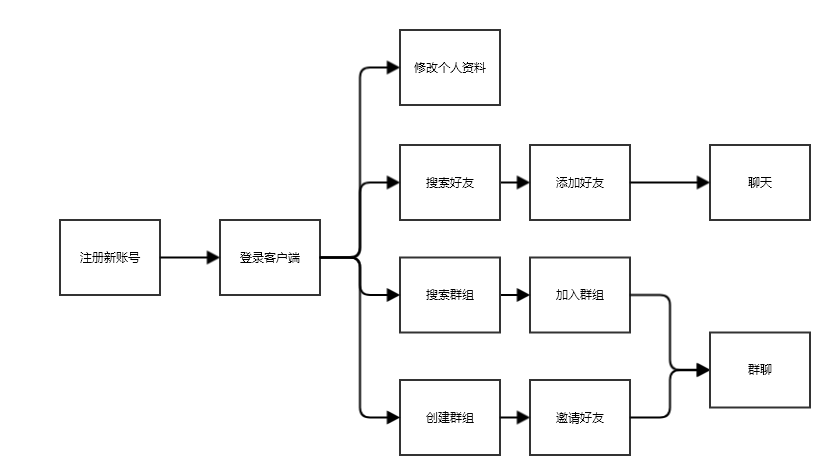
\includegraphics[width=13cm]{base_flowchart}
	\caption{总体流程图} \label{fig:base_flowchart}
\end{figure}

%\subsection{系统基本流程}
%此处应当有一个图和对应的描述。

\subsection{客户端基本流程}
%这只是举个例子,如果没有客户端则不需要此节。
\begin{figure}[h]
	\centering
	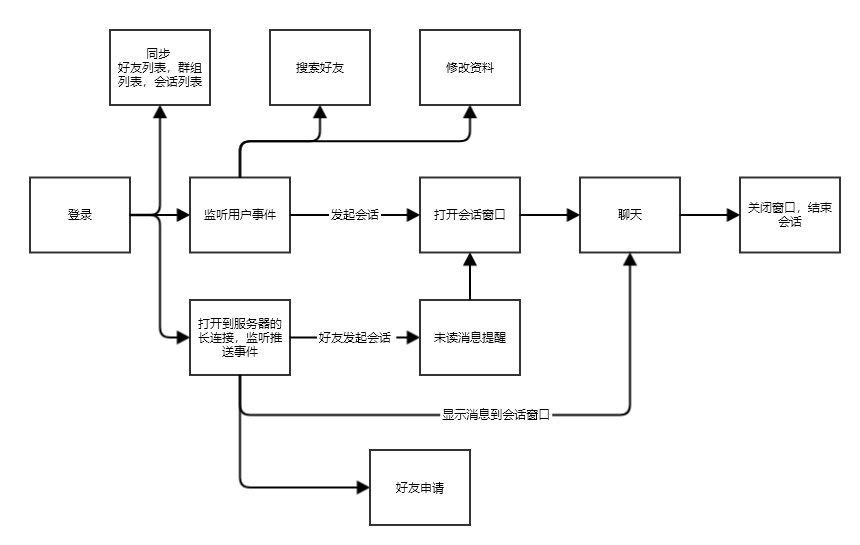
\includegraphics[width=13cm]{client_flowchart}
	\caption{客户端流程图} \label{fig:client_flowchart}
\end{figure}
用户在登陆账号后,客户端会从服务器同步好友,群组和会话信息。并打开一个到服务器的长连接,监听服务器的推送消息。
用户可以点击好友列表或群组列表中的项目启动一个会话窗口,在会话窗口中发送各种消息。
服务器会及时推送消息给客户端,客户端会将消息及时显示到对应的窗口中。
客户端也提供好友搜索,个人资料修改等功能。

\subsection{服务器端基本流程}
%这只是举个例子,如果没有服务器端则不需要此节。
\begin{figure}[h]
	\centering
	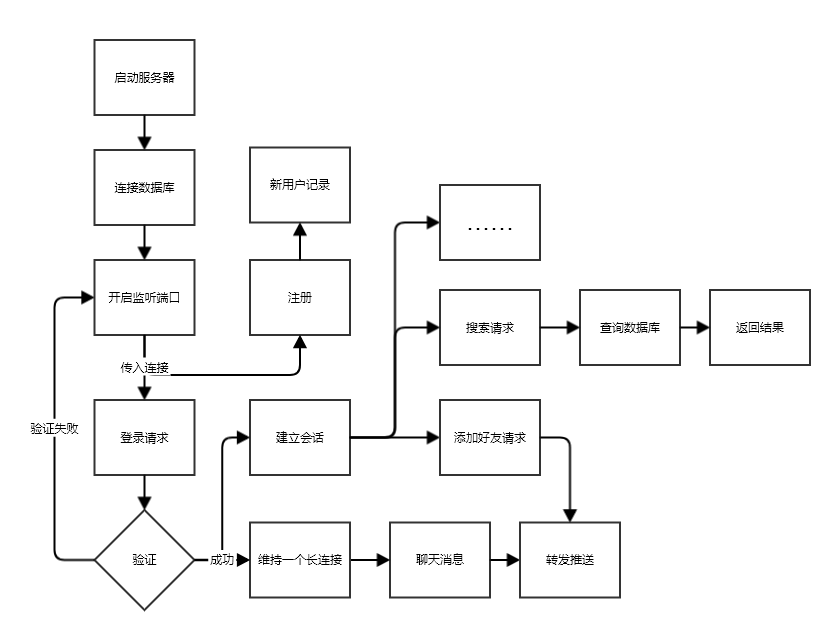
\includegraphics[width=13cm]{server_flowchart}
	\caption{服务端流程图} \label{fig:server_flowchart}
\end{figure}

服务端启动后连接数据库,监听端口,响应来自客户端的请求。
处理注册请求,验证合法后向数据库插入一条新纪录。
处理登陆请求,验证合法后为该账号分配一个 session 对象,
并维持一条到客户端的长连接,聊天消息,好友请求都会从该连接推送给客户端。
服务端亦提供 http api,用于修改个人资料,查找用户等功能。

\subsection{功能1具体流程}
举个例子:交易处理流程

已登录用户在购物车中提交请求交易的 POST 请求,提交的表单中指明了交易中包括的
所有商品、商家、付款信息、收货地址,输入输出处理系统接收到合法请求后,向商品信息
系统请求数据,收到数据以后验证是否正确,然后向订单系统发起生成新订单的请求,订单
系统负责更新商品信息系统、商家信息,通知商家接单,返回订单处理结果输入输出处理系
统,输入输出处理系统依照结果产生 HTML 页面,并返回给用户。

\subsection{登录功能具体流程}
%此处应当有描述。
\begin{figure}[h]
	\centering
	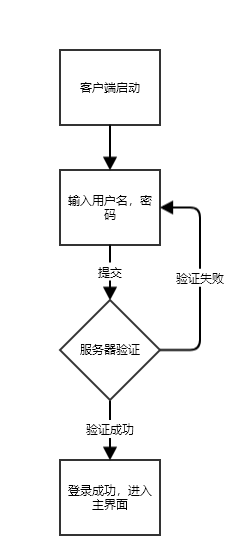
\includegraphics[width=5cm]{login_flowchart}
	\caption{登录功能流程图} \label{fig:login_flowchart}
\end{figure}
用户打开客户端,输入用户名和密码,点击登录提交至服务器,服务器查询数据库验证用户名密码是否合法。
若合法则进入主界面,否则提示用户出错。

\subsection{用户搜索功能具体流程}
%此处应当有一个描述。
\begin{figure}[h]
	\centering
	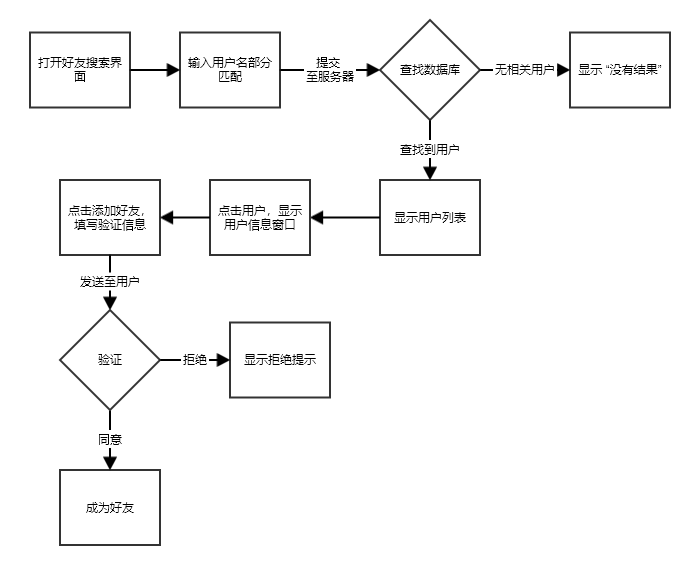
\includegraphics[width=13cm]{search_friend_flowchart}
	\caption{用户搜索功能流程图} \label{fig:search_friend_flowchart}
\end{figure}
用户打开搜索窗口,在搜索框输入要搜索的内容,一般是用户名的部分匹配。点击按钮提交给服务器。
服务器获取参数后查询数据库,获取返回结果,若无记录,则返回错误代码,客户端收到响应后显示无结果。
否则客户端将收到的用户数据以列表形式显示出来。
用户可以点击搜索结果中的项目打开用户信息窗口,添加好友。

\subsection{聊天功能具体流程}
用户在客户端的好友列表或群组列表选择项目,打开会话窗口,即可发送文本,图片或者语音消息。
消息数据会通过长连接发送给服务器。
服务器在接收到消息后就会推送给相应的用户。如果是群聊,则广播给所有群成员。
其他客户端收到后,若之前并未打开会话窗口,则会收到消息提醒。
若会话窗口已打开,则消息内容会显示到会话窗口中。
消息本身也将保存在服务器的数据库中。
不在线的用户上线后,服务器会推送未读的消息给客户端。

\section{功能结构设计}
\subsection{整体结构}
%此处应当有一个图和对应的描述。系统如果像微内核那样,划分成核心模块和若干个子系统,此处应当有图示及说明,然后后续几个节应当描述这几个子系统。如果系统像宏内核,那应当说明有哪些紧密联系的模块,并在后续几个节内描述这些模块。

\begin{figure}[h]
	\centering
	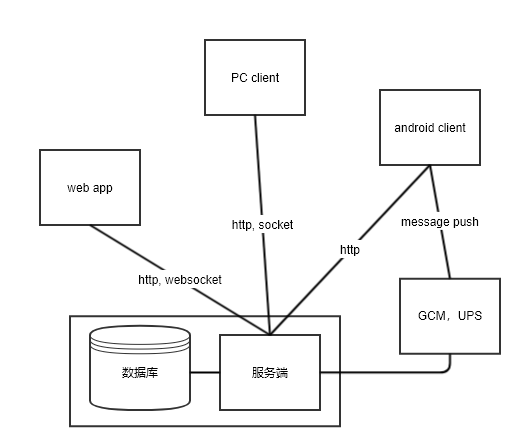
\includegraphics[width=13cm]{overall_architecture}
	\caption{整体结构} \label{fig:overall_architecture}
\end{figure}

\subsection{用户端结构}
此处应当有一个图和对应的描述。这只是举个例子。可能的内容包括用户端的具体模块、耦合情况等。

\subsection{服务器端结构}
此处应当有一个图和对应的描述。这只是举个例子。

\subsection{后台数据库维护模块结构}
此处应当有一个图和对应的描述。这只是举个例子。



\section{功能需求与程序代码的关系}
[此处指的是不同的需求分配到哪些模块去实现。可按不同的端拆分此表]
\begin{table}[htbp]
\centering
\caption{功能需求与程序代码的关系表} \label{tab:requirement-module}
\begin{tabular}{|c|c|c|c|}
    \hline
    · & 模块1 & 模块2 & 模块3 \\
    \hline
    需求1 & · & Y & · \\
    \hline
    需求2 & · & Y & · \\
    \hline
    需求3 & · & Y & · \\
    \hline
    需求4 & Y & · & · \\
    \hline
    需求5 & · & · & Y \\
    \hline
\end{tabular}
\note{各项功能需求的实现与各个程序模块的分配关系}
\end{table}
\chapter{接口设计}
\section{数据类型}
本节描述各API会用到的数据结构类型。所有POST请求的上传内容,以及响应内容均为JSON格式。
\subsection{符号说明}
\begin{itemize}
    \item  *: 必填
    \item  !: 只读(只会出现在响应内容)
    \item  ?: 可选
    \item  \&: 只写(只会出现在请求的上传内容)
\end{itemize}
\subsection{DateTime}
用零时区存储的符合ISO-8601标准的日期时间字符串。如:2018-05-12T07:12:29.181605Z。
\subsection{User}
\begin{lstlisting}[language=C]
{
    id!: Number,
    last_login!: DateTime | null,
    username: String,
    email: Email,
    description: String,
    avatar_url!: URL,
    address: String,
    site_url: URL,
    description: String
}
\end{lstlisting}
\subsection{Message}
用来表示一条消息。此类型可被扩展以支持语音等多媒体消息。
\begin{lstlisting}[language=C]
{
    id!: Number,
    category!: String,
    user_id*: Number, //发送方的用户ID
    message*: String, // 消息内容
    has_read!: Boolean, // 对方是否已读
    created!: DateTime // 发送时间
}
\end{lstlisting}


\section{外部接口}
服务器对外公开的HTTP API遵循RESTful API设计规范。即,对于相同URL的请求,不同的请求方法(如POST, GET, PUT, DELETE等),往往对应着较为统一、类似的语义。

具体而言,标 API<T> <base> 的为类型 T 的 CRUD API, 操作有如下几类:(每个操作均对应到一个HTTP请求方法)
\begin{itemize}
    \item list : GET <base> -> Page<T>
    \item create : POST <base> -> T
    \item retrieve: GET <base>/<id>/ -> T
    \item update : PUT <base>/<id>/ -> T (输入为 T,完整更新对象)
    \item patch : PATCH <base>/<id>/ -> T (输入为 T?,局部更新对象)
    \item delete : DELETE <base>/<id>/
\end{itemize}

本系统主要包含的HTTP API如下:
\subsection{用户相关}
\subsubsection{\textbf{API<User>} /chat/users}
\textbf{请求方法}
\begin{itemize}
    \item GET

        (要求登录)列出符合条件的用户。由搜索功能调用。

        \textbf{查询参数:}
        \begin{itemize}
            \item username: 字符串,表示用户名,或要查询的用户名的部分匹配
        \end{itemize}
        \textbf{返回结果:}
        \begin{itemize}
            \item 200: 操作成功。
            \item 403: 未登录。
        \end{itemize}
    \item POST
        
        创建一个新用户。

        POST数据的格式为User数据类型,需要提供所有必填的数据项。

        \textbf{返回结果:}
        \begin{itemize}
            \item 200: 操作成功,并自动登录。
            \item 404: 当前已有用户登录。
        \end{itemize}

    \item PATCH
        
        (要求登录)更新用户自己的部分信息,

        POST数据的格式为User数据类型的部分数据项。

        \textbf{返回结果:}
        \begin{itemize}
            \item 200: 操作成功。
            \item 403: 未登录,或试图修改其他用户的信息。
        \end{itemize}

\end{itemize}

\subsubsection{\textbf{POST} /chat/users/login}
用户登录。

\textbf{输入:}
\begin{lstlisting}[language=C]
    {
        username*: String,
        password*: String
    }
\end{lstlisting}

\textbf{返回结果:}
\begin{itemize}
    \item 200: 操作成功。
    \item 404: 当前已有用户登录。
    \item 403: 认证失败,即密码错误。
\end{itemize}

\subsubsection{\textbf{GET} /chat/users/logout}
(要求登录)用户登出。
\textbf{返回结果:}
\begin{itemize}
    \item 200: 操作成功。
    \item 403: 未登录。
\end{itemize}

\subsubsection{\textbf{GET} /chat/users/friends}
(要求登录)获取好友列表。

\textbf{查询参数:}
\begin{itemize}
    \item (可选)username: 字符串,表示需要查询的好友的用户名,或其部分匹配。
    \item (可选)group\_id: 分组id,将queryset限定为group\_id所指定的分组内的好友。
\end{itemize}

\textbf{返回结果:}
\begin{itemize}
    \item 200 - 操作成功,并返回由User数据类型组成的列表。
    \item 404 - 未找到给定条件的用户。
    \item 403 - 未登录。
\end{itemize}
    

\subsubsection{\textbf{POST} /chat/users/<username>/follow}
(要求登录)请求添加用户名为username的用户为好友。

\textbf{返回结果:}
\begin{itemize}
    \item 200: 请求发送成功。
    \item 403: 未登录。
    \item 404: 未找到用户名为username的用户。
\end{itemize}

\subsubsection{\textbf{POST} /chat/users/<username>/unfollow}
(要求登录)删除用户名为username的好友。
\textbf{返回结果:}
\begin{itemize}
    \item 200: 操作成功完成。
    \item 403: 未登录。
    \item 404: 未找到用户名为username的用户。
\end{itemize}

\subsection{消息相关}
\subsubsection{\textbf{API<Message>} /chat/messages}
\textbf{请求方法}
\begin{itemize}
    \item GET
    获取所有与好友的消息列表。

    \textbf{查询参数:}
    \begin{itemize}
        \item anchor: DateTime类型,用来指明此时间戳以后的消息需要接收。
    \end{itemize}

    \textbf{返回结果:}
    \begin{itemize}
    \item 200: 操作成功完成,并返回由Message数据类型组成的列表。
    \item 403: 未登录。
    \end{itemize}
    \item POST
    发送一条消息。

    \textbf{输入:}
    \begin{lstlisting}[language=C]
    {
        client_type: String, // 发送方使用的客户端名称
        sender: Number, // 发送方的用户ID
        message_type_name: String, // 消息类型
        content: String, // 消息内容
        send_to: String // 由逗号分隔的接收人ID列表
    }
    \end{lstlisting}
\end{itemize}

\chapter{数据结构设计}
\section{逻辑结构设计}
% \subsection{用户管理系统数据结构设计}
%讲述本系统内需要什么数据结构。这指的是程序运行过程中维护的数据结构。只是举个例子,此处应和3.3一致。

\subsection{客户端数据结构}

\subsubsection{好友列表}
客户端需要从服务器拉取自己的好友并维持在本地,并记录好友的在线状态。
用户界面使用该数据结构填充好友列表控件。

\subsubsection{群组列表}
客户端需要从服务器拉取自己的群组并维持在本地,
用户界面使用该数据结构填充群组列表控件。

\subsubsection{消息记录}
用户每一个的群组和好友都会有一份消息记录。
用户界面使用该数据结构填充消息框控件。

\subsubsection{输入缓冲}
对应用户的文本输入

\subsection{服务端数据结构}

\subsubsection{会话池}
对每一个客户端都需要维持一个长连接。
使用一个会话池来维护连接对象。

\subsubsection{路由表}
记录了 url 到内部接口的映射


%\section{物理结构设计}
%各数据结构无特殊物理结构要求。(如果有,比如说hadoop等,应当具体说明)

\section{数据结构与程序模块的关系}
[此处指的是不同的数据结构分配到哪些模块去实现。可按不同的端拆分此表]
\begin{table}[htbp]
\centering
\caption{数据结构与程序代码的关系表} \label{tab:datastructure-module}
\begin{tabular}{|c|c|c|c|}
    \hline
    · & 模块1 & 模块2 & 模块3 \\
    \hline
    结构1 & · & Y & · \\
    \hline
    结构2 & · & Y & · \\
    \hline
    结构3 & · & Y & · \\
    \hline
    结构4 & Y & · & · \\
    \hline
    结构5 & · & · & Y \\
    \hline
\end{tabular}
\note{各项数据结构的实现与各个程序模块的分配关系}
\end{table}
\chapter{数据库设计}
\section{数据库环境说明}
%本系统的数据系统采用MySQL/PostgreSQL/Microsoft SQL Server数据库系统。

%其中xxx模块因为xxx而需要用到Hadoop架构。

本系统的数据系统采用MySQL数据库系统。

\section{数据库的命名规则}
%是否允许单词缩写,允许的单词缩写有哪些。
允许单词缩写
identity - ID
password - pw

表名是单数还是复数。关联表如何命名。字符数限制等。

% 字段是否带上前缀(如integer类型则加上i前缀等)。不带

\section{逻辑设计}
%是否需要满足某一种范式。
逻辑设计满足 BCNF

画个实体的逻辑关系表/图在此处。

\section{物理设计}
\subsection{数据库产品}
%用哪家数据库,是否分布式等。
mysql

\subsection{实体属性、类型、精度}
\subsubsection{客户数据表设计}
\begin{table}[htbp]
\centering
\caption{用户数据表Users设计} \label{tab:client-database}
\begin{tabular}{|c|c|c|c|c|}
    \hline
    字段名 & 类型 & 大小 & 说明 & 备注 \\
    \hline
    ID & char & 64 & 用户的唯一标识符 & 主键\\
    \hline
    pw & char & 512 & 用户的登录密码hash值 & · \\
    \hline
    email & char & 64 & 用户的注册邮箱 & 唯一 \\
    \hline
    last_login & time & 16 & 最近登录时间 & · \\
    \hline
    register_time & time & 16 & 注册时间 & · \\
    \hline
    birthday & date & 16 & 生日 & · \\
    \hline
    sex & char & 4 & 性别 & · \\
    \hline
\end{tabular}
\note{用户数据表Users设计}
\end{table}

\subsubsection{订单数据表设计}
\begin{table}[htbp]
\centering
\caption{订单数据表Orders设计} \label{tab:order-database}
\begin{tabular}{|c|c|c|c|c|}
    \hline
    字段名 & 类型 & 大小 & 说明 & 备注 \\
    \hline
    ID & char & 64 & 订单的唯一标识符 & 主键\\
    \hline
    user & char & 64 & 对应用户 & 外键,来自xx表 \\
    \hline
\end{tabular}
\note{订单数据表Orders设计}
\end{table}
\section{安全性设计}
%备份和容灾设计。
本产品的服务端主要面向有自己搭建即时通讯服务需求的个人用户和中小企业用户,
预期使用规模较小,所以没有特别的容灾设计,
数据备份工作依靠服务端维护人员自行开展。

\section{数据库管理与维护说明}
对于数据库的维护,随时对数据库中的信息加以调试和保存备份。同样需要个工作人员进行系统的分析和用户的反馈,对系统进行升级以及功能的完善。同时保证系统安全有序的运行。
\chapter{界面设计}
\section{客户端界面}
% 此处应当有一个简略的图,重点是展示你与用户交互的逻辑。(processon上画一个不花时间)
\begin{figure}[h]
	\centering
	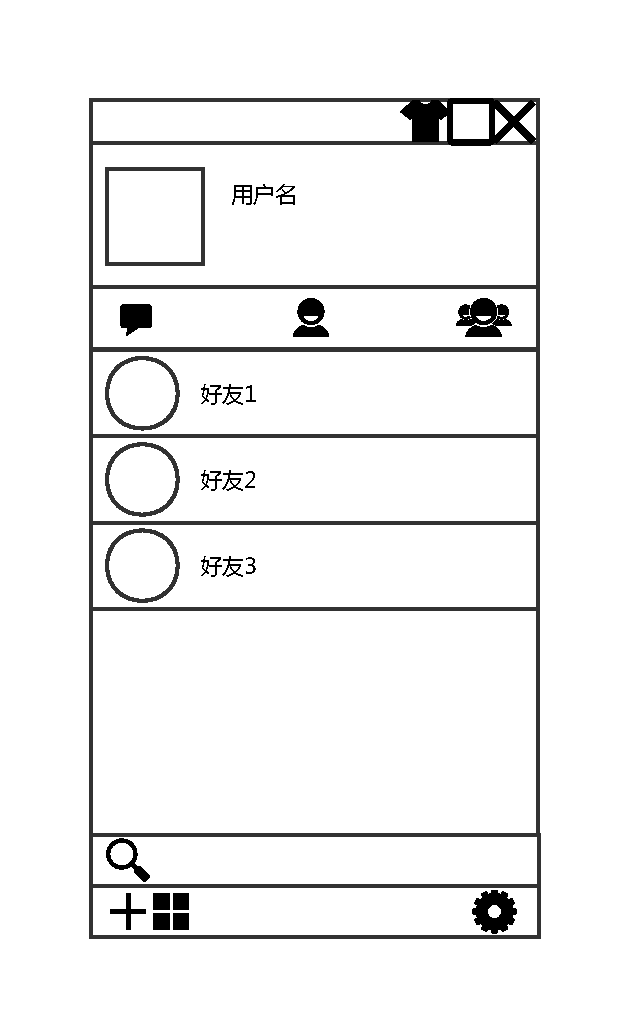
\includegraphics[width=10cm]{main_ui}
	\caption{主界面} \label{fig:main_ui}
\end{figure}


最上方显示自己的头像和用户名。
中间有三个标签页,从左到右分别是会话,好友和群组。
下方有一个搜索框,可用于搜索已添加的好友。
最下方的三个按钮的功能分别是添加新好友,菜单和设置。

见图-\ref{fig:main_ui}

\begin{figure}[h]
	\centering
	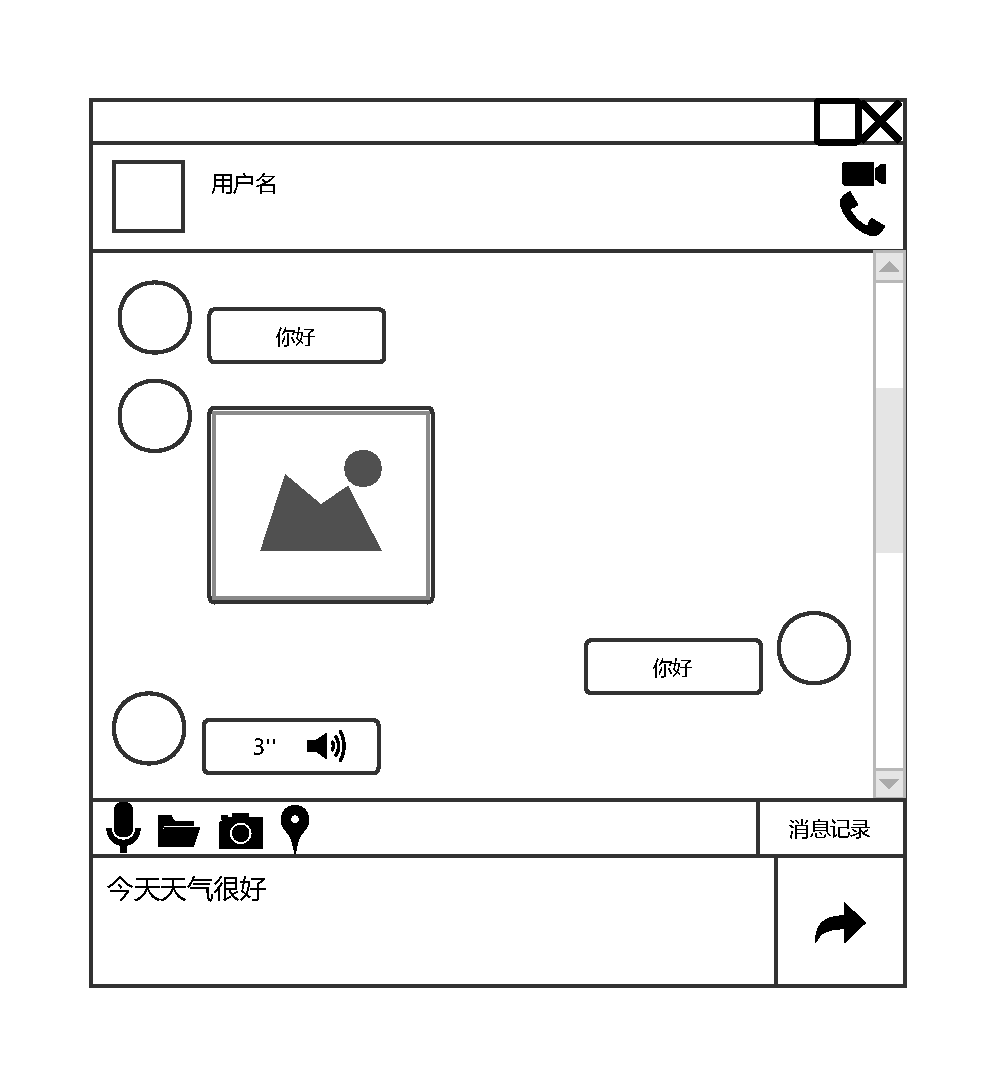
\includegraphics[width=10cm]{chat_ui}
	\caption{聊天界面} \label{fig:chat_ui}
\end{figure}


最上方显示对方的头像和用户名(或群的头像和群名),左侧可以开启视频或语音聊天。
中间为消息显示区,消息放在气泡中显示,自己的消息在右侧,其他人的在左侧。
最下方为文本输入框,左侧为发送按钮。
输入框上方为工具栏,可以用于发送图片和语音消息,可以查看聊天记录。

见图-\ref{fig:chat_ui}

\section{服务器端界面}
% 此处应当有一个简略的图。

\begin{figure}[h]
	\centering
	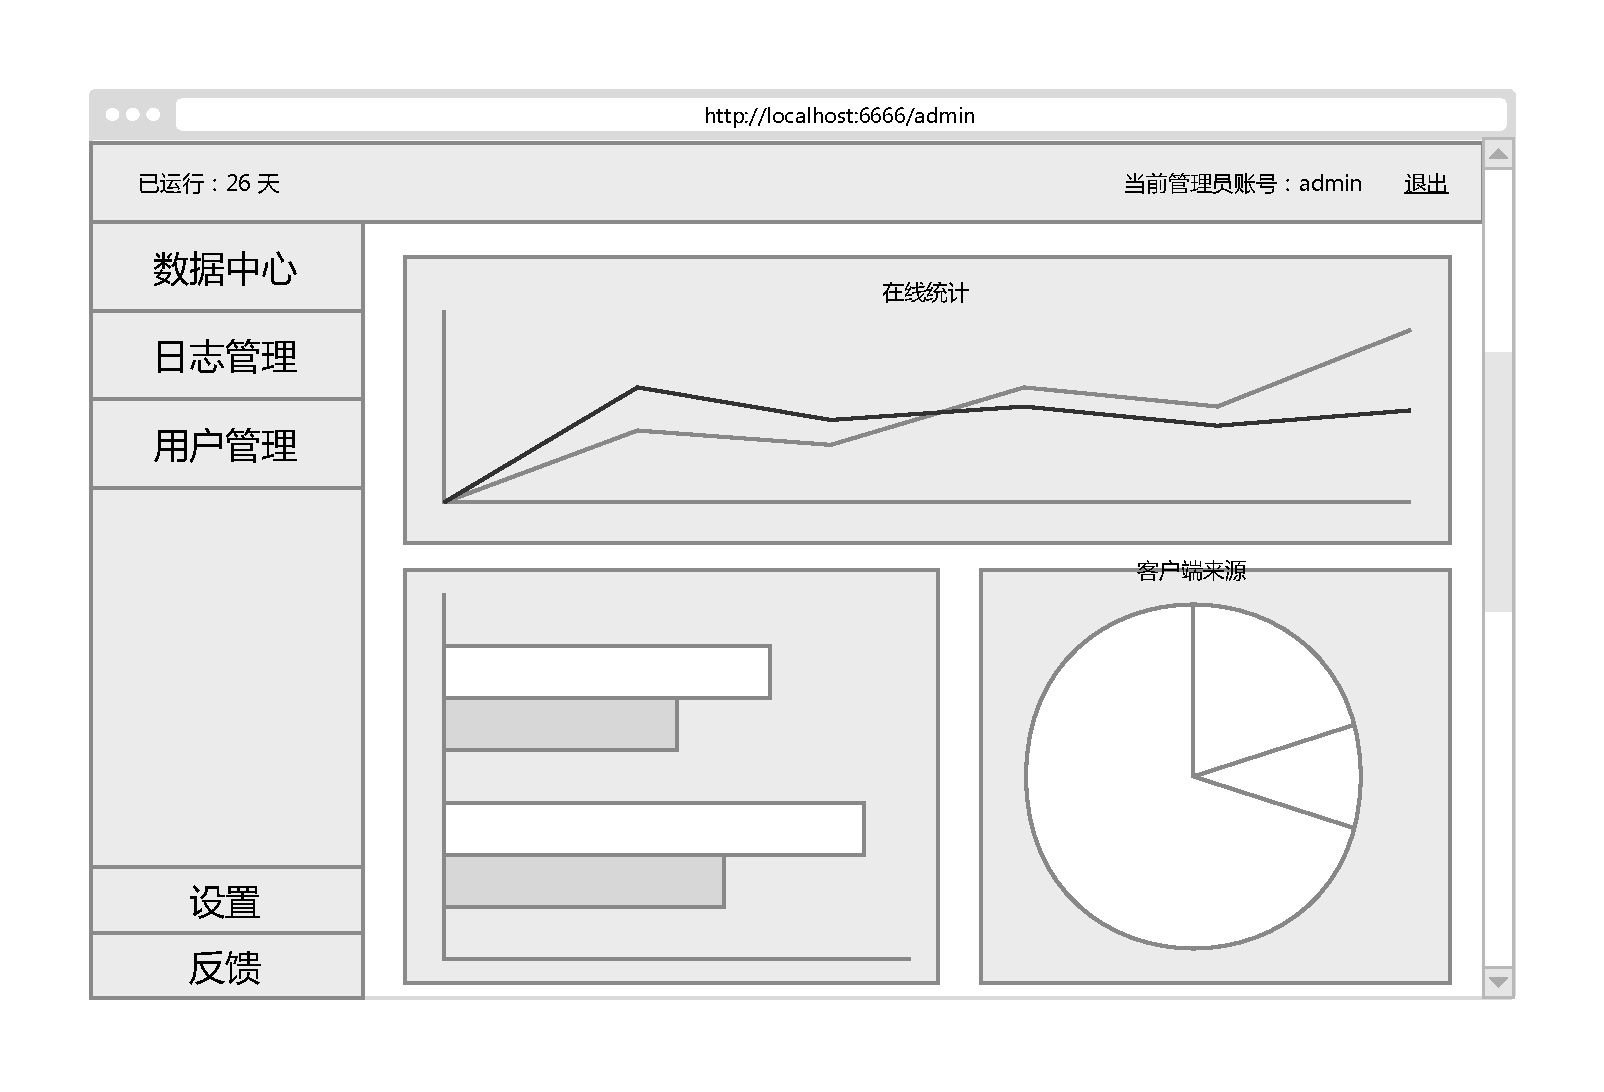
\includegraphics[width=13cm]{admin_ui}
	\caption{服务器端界面} \label{fig:admin_ui}
\end{figure}

服务端提供一个web管理接口,管理员可以通过浏览器打开。
web接口提供日志查看,数据统计,账号管理等功能。

见图-\ref{fig:admin_ui}


\section{登录界面}
% 此处应当有一个简略的图。

\begin{figure}[h]
	\centering
	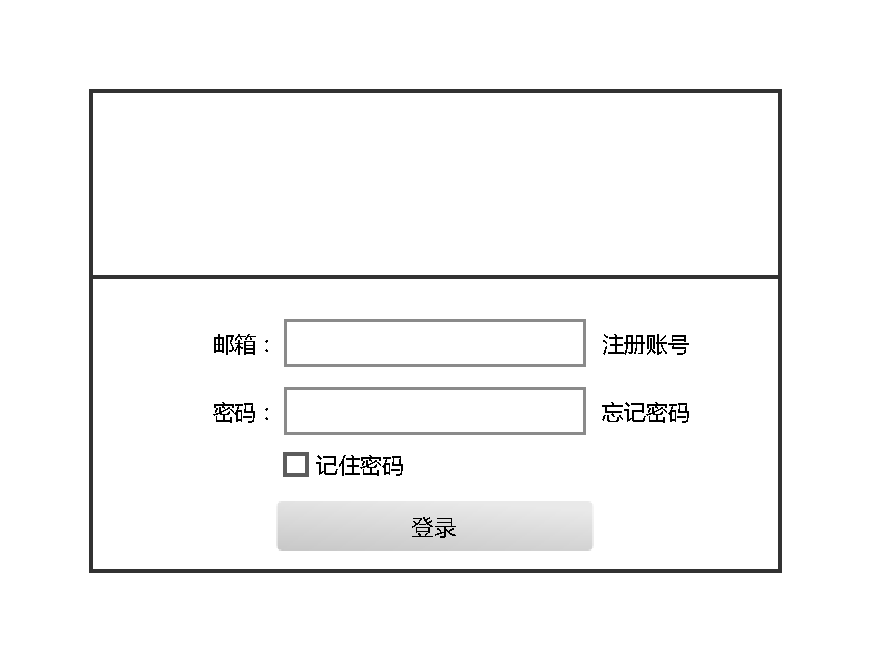
\includegraphics[width=13cm]{login_ui}
	\caption{登录界面} \label{fig:login_ui}
\end{figure}

输入邮箱密码登陆,可选择记住密码,右侧有注册账号和忘记密码的按钮。
界面上方放置banner图片,增加美观。

见图-\ref{fig:login_ui}


\section{用户搜索功能界面}
\begin{figure}[h]
	\centering
	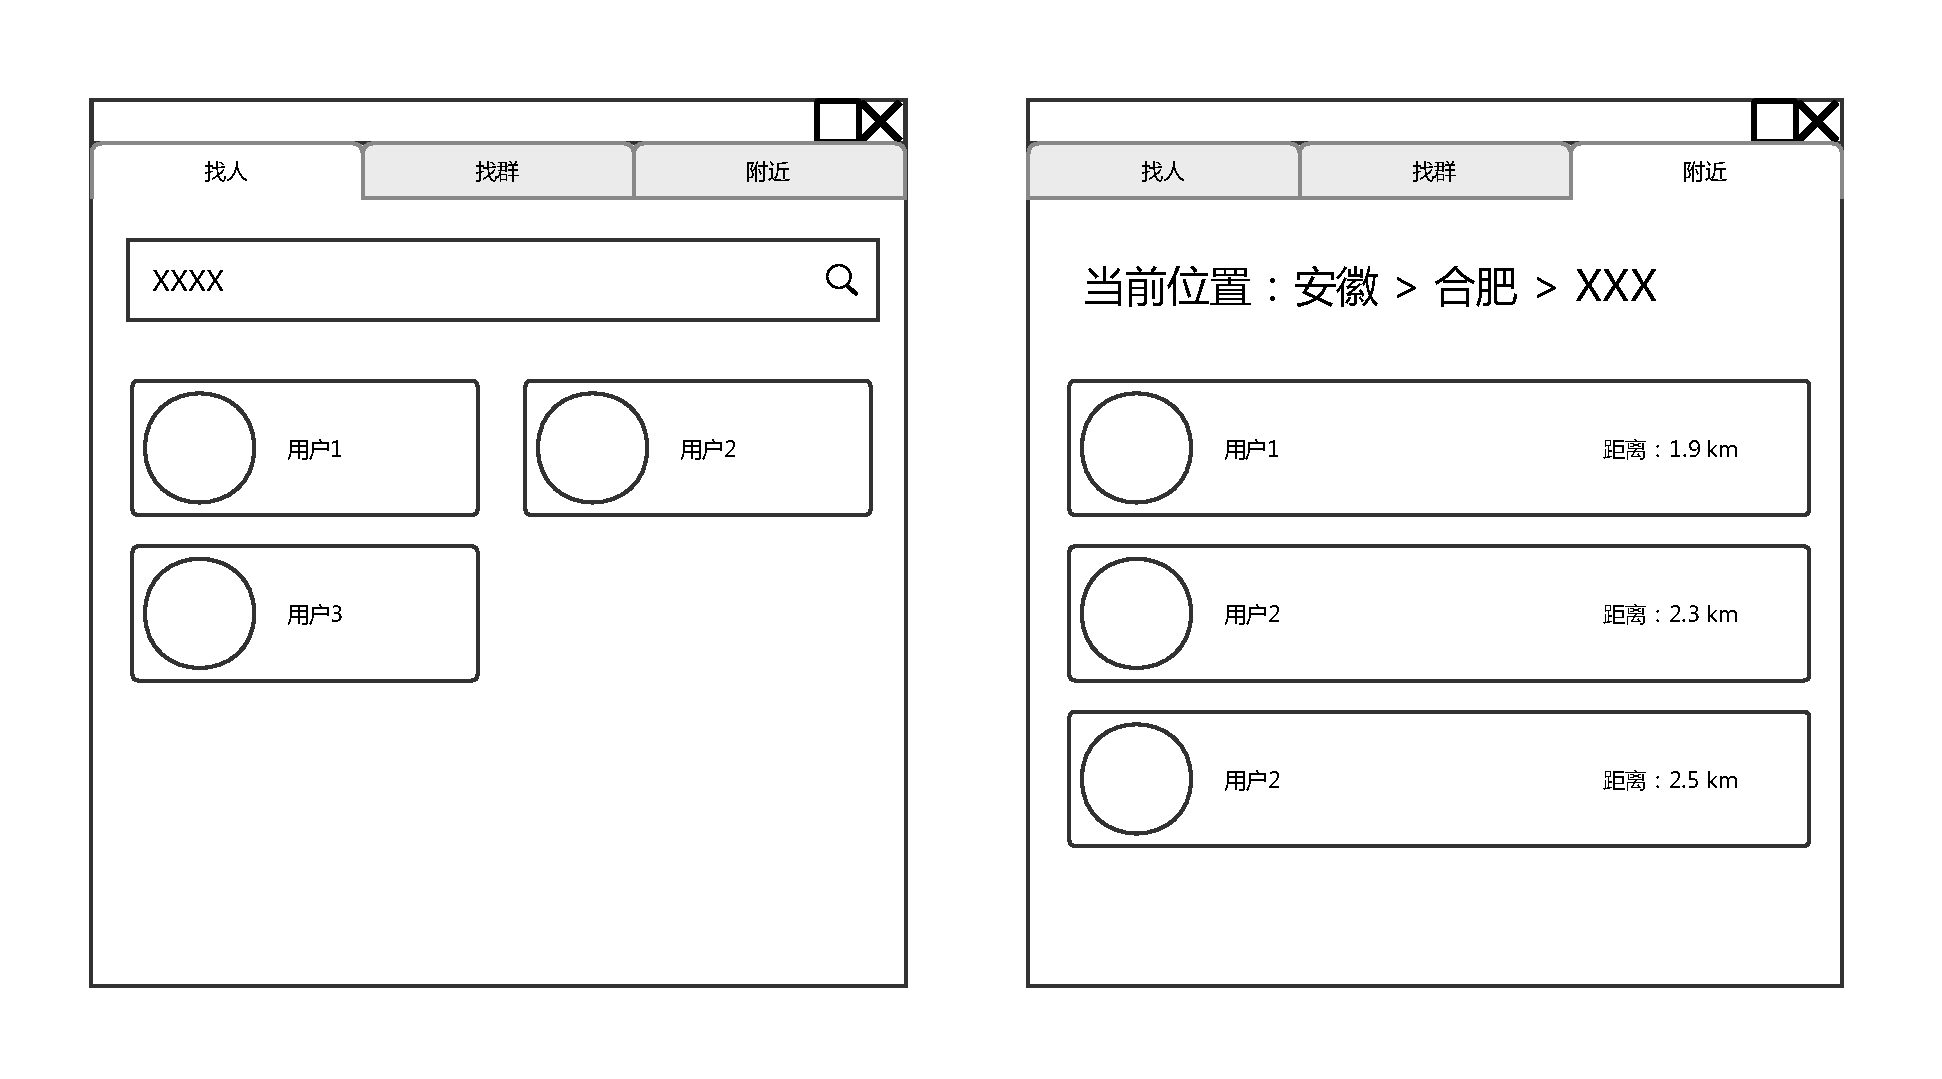
\includegraphics[width=15cm]{search_friend_ui}
	\caption{用户搜索界面} \label{fig:search_friend_ui}
\end{figure}

共三个标签页可用于搜人,搜群,附近。
找人,找群标签页在搜索框输入内容后显示结果。
附近标签页显示了当前位置和附近的用户以及估计的距离。
点击用户弹出用户信息界面。

见图-\ref{fig:search_friend_ui}

\chapter{出错处理设计}
\section{出错信息}
建立错误信息表,针对可能出现的错误为其制定错误信号输出、错误含义解释、错误解决方法和相应的客户端提示。

\section{补救措施}
\subsection{数据库出错}
对于此即时通讯软件,数据库主要存储用户信息和各种通讯记录。若是数据库相关软件出错,则回滚软件至稳定可用的版本,再处理软件错误;若是数据库相关硬件如存储介质出错导致数据库信息破坏,则暂停系统服务,使用最近未出错的备份数据,结合所记录的客户端数据流将其同步更新至当前状态再投入使用。

\subsection{某模块失效处理}
使用另一个效率稍低的但是稳定的系统,虽然其提供更少的服务,但其也能进行数据库的实时备份。这样在失效模块处理完成后,可以很快的进行数据同步,同时也可以很快的进行原系统的运行。

\chapter{安全保密设计}
\begin{itemize}
\item 数据库服务器保护:

用户或管理者只会获得能完成他们操作所需的最小权限,以避免越界访问和修改。
\item 安全数据传输:

客户端与服务器之间的数据传输使用HTTPS进行加密。默认情况下,所有服务都可以通过本地主机连接或使用加密的SSL连接相互通话。

\item 用户密码:

用户设定密码时,使用流行的zxcvbn库检查密码的强度。拒绝弱密码,鼓励强密码。并使用PBKDF2算法存储用户密码。


\end{itemize}

\chapter{维护设计}
可能的内容包括数据库的日常备份、压缩、维护等。

%\chapter{图片}
本章展示图片相关用法。

\section{示例}
\begin{figure}[ht]
\centering

\includegraphics[width=10cm]{ustc_logo_fig}
\caption{测试图片} \label{fig:figure1}
\end{figure}

\section{带图注的图}
\begin{figure}[ht]
\centering

\includegraphics[width=10cm]{ustc_logo_fig}
\caption{带图注的图片}\label{fig:noted-figure}
\note{the solid lines represent the time histogram of the spontaneous activities of an old monkey cell(gray) and a young monkey cell (black). The bin-width is 1}
\end{figure}

%\chapter{表格}

\section{A Simple Table}
\begin{table}[htbp]
\centering
\caption{这里是表的标题} \label{tab:simpletable}
\begin{tabular}{|c|c|}
    \hline
    a & b \\
    \hline
    c & d \\
    \hline
\end{tabular}
\note{这里是表的注释}
\end{table}

\section{长表格}
\begin{longtable}{ccc}
% 首页表头
\caption[长表格演示]{长表格演示} \label{tab:longtable} \\
\toprule[1.5pt]
名称  & 说明 & 备注\\
\midrule[1pt]
\endfirsthead
% 续页表头
\caption[]{长表格演示(续)} \\
\toprule[1.5pt]
名称  & 说明 & 备注 \\
\midrule[1pt]
\endhead
% 首页表尾
\hline
\multicolumn{3}{r}{\small 续下页}
\endfoot
% 续页表尾
\bottomrule[1.5pt]
\endlastfoot

AAAAAAAAAAAA   &   BBBBBBBBBBB   &   CCCCCCCCCCCCCC   \\
AAAAAAAAAAAA   &   BBBBBBBBBBB   &   CCCCCCCCCCCCCC   \\
AAAAAAAAAAAA   &   BBBBBBBBBBB   &   CCCCCCCCCCCCCC   \\
AAAAAAAAAAAA   &   BBBBBBBBBBB   &   CCCCCCCCCCCCCC   \\
AAAAAAAAAAAA   &   BBBBBBBBBBB   &   CCCCCCCCCCCCCC   \\
AAAAAAAAAAAA   &   BBBBBBBBBBB   &   CCCCCCCCCCCCCC   \\
AAAAAAAAAAAA   &   BBBBBBBBBBB   &   CCCCCCCCCCCCCC   \\
AAAAAAAAAAAA   &   BBBBBBBBBBB   &   CCCCCCCCCCCCCC   \\
AAAAAAAAAAAA   &   BBBBBBBBBBB   &   CCCCCCCCCCCCCC   \\
AAAAAAAAAAAA   &   BBBBBBBBBBB   &   CCCCCCCCCCCCCC   \\
AAAAAAAAAAAA   &   BBBBBBBBBBB   &   CCCCCCCCCCCCCC   \\
AAAAAAAAAAAA   &   BBBBBBBBBBB   &   CCCCCCCCCCCCCC   \\
AAAAAAAAAAAA   &   BBBBBBBBBBB   &   CCCCCCCCCCCCCC   \\
AAAAAAAAAAAA   &   BBBBBBBBBBB   &   CCCCCCCCCCCCCC   \\
AAAAAAAAAAAA   &   BBBBBBBBBBB   &   CCCCCCCCCCCCCC   \\
AAAAAAAAAAAA   &   BBBBBBBBBBB   &   CCCCCCCCCCCCCC   \\
AAAAAAAAAAAA   &   BBBBBBBBBBB   &   CCCCCCCCCCCCCC   \\
AAAAAAAAAAAA   &   BBBBBBBBBBB   &   CCCCCCCCCCCCCC   \\
AAAAAAAAAAAA   &   BBBBBBBBBBB   &   CCCCCCCCCCCCCC   \\
AAAAAAAAAAAA   &   BBBBBBBBBBB   &   CCCCCCCCCCCCCC   \\
AAAAAAAAAAAA   &   BBBBBBBBBBB   &   CCCCCCCCCCCCCC   \\
AAAAAAAAAAAA   &   BBBBBBBBBBB   &   CCCCCCCCCCCCCC   \\
AAAAAAAAAAAA   &   BBBBBBBBBBB   &   CCCCCCCCCCCCCC   \\
AAAAAAAAAAAA   &   BBBBBBBBBBB   &   CCCCCCCCCCCCCC   \\
AAAAAAAAAAAA   &   BBBBBBBBBBB   &   CCCCCCCCCCCCCC   \\
AAAAAAAAAAAA   &   BBBBBBBBBBB   &   CCCCCCCCCCCCCC   \\
AAAAAAAAAAAA   &   BBBBBBBBBBB   &   CCCCCCCCCCCCCC   \\
AAAAAAAAAAAA   &   BBBBBBBBBBB   &   CCCCCCCCCCCCCC   \\
AAAAAAAAAAAA   &   BBBBBBBBBBB   &   CCCCCCCCCCCCCC   \\
AAAAAAAAAAAA   &   BBBBBBBBBBB   &   CCCCCCCCCCCCCC   \\
AAAAAAAAAAAA   &   BBBBBBBBBBB   &   CCCCCCCCCCCCCC   \\
AAAAAAAAAAAA   &   BBBBBBBBBBB   &   CCCCCCCCCCCCCC   \\
AAAAAAAAAAAA   &   BBBBBBBBBBB   &   CCCCCCCCCCCCCC   \\
AAAAAAAAAAAA   &   BBBBBBBBBBB   &   CCCCCCCCCCCCCC   \\
AAAAAAAAAAAA   &   BBBBBBBBBBB   &   CCCCCCCCCCCCCC   \\
AAAAAAAAAAAA   &   BBBBBBBBBBB   &   CCCCCCCCCCCCCC   \\
\end{longtable}

%\chapter{算法环境}
模板中使用 \texttt{algorithm2e} 宏包实现算法环境。关于该宏包的具体用法,
请阅读宏包的官方文档。

\begin{algorithm}[htbp]
\SetAlgoLined
\KwData{this text}
\KwResult{how to write algorithm with \LaTeX2e }

initialization\;
\While{not at end of this document}{
    read current\;
    \eIf{understand}{
        go to next section\;
        current section becomes this one\;
    }{
        go back to the beginning of current section\;
    }
}
\caption{算法示例1}
\label{algo:algorithm1}
\end{algorithm}

\IncMargin{1em}
\begin{algorithm}
\SetKwData{Left}{left}\SetKwData{This}{this}\SetKwData{Up}{up}
\SetKwFunction{Union}{Union}\SetKwFunction{FindCompress}{FindCompress}
\SetKwInOut{Input}{input}\SetKwInOut{Output}{output}

\Input{A bitmap $Im$ of size $w\times l$}
\Output{A partition of the bitmap}
\BlankLine
\emph{special treatment of the first line}\;
\For{$i\leftarrow 2$ \KwTo $l$}{
    \emph{special treatment of the first element of line $i$}\;
    \For{$j\leftarrow 2$ \KwTo $w$}{\label{forins}
        \Left$\leftarrow$ \FindCompress{$Im[i,j-1]$}\;
        \Up$\leftarrow$ \FindCompress{$Im[i-1,]$}\;
        \This$\leftarrow$ \FindCompress{$Im[i,j]$}\;
        \If(\tcp*[h]{O(\Left,\This)==1}){\Left compatible with \This}{\label{lt}
            \lIf{\Left $<$ \This}{\Union{\Left,\This}}
            \lElse{\Union{\This,\Left}}
        }
        \If(\tcp*[f]{O(\Up,\This)==1}){\Up compatible with \This}{\label{ut}
        \lIf{\Up $<$ \This}{\Union{\Up,\This}}
        \tcp{\This is put under \Up to keep tree as flat as possible}\label{cmt}
        \lElse{\Union{\This,\Up}}\tcp*[h]{\This linked to \Up}\label{lelse}
        }
    }
    \lForEach{element $e$ of the line $i$}{\FindCompress{p}}
}
\caption{算法示例2}\label{algo_disjdecomp}
\label{alog:algorithm2}
\end{algorithm}\DecMargin{1em}

%\chapter{代码环境}
模板中使用 \texttt{listings} 宏包实现代码环境。详细用法见宏包的官方说明文档。

以下是代码示例,可以在文中任意位置引用\autoref{first-code} 。
\begin{lstlisting}[language=C, caption=示例代码, label={code:first-code}]
#include <stdio.h>

int main( )
{
    printf("hello, world\n");
    return 0;
}
\end{lstlisting}

%\chapter{引用文献标注}

\section{著者-出版年制标注法}

\noindent
\verb|\citestyle{ustcauthoryear}|
\citestyle{ustcauthoryear}

\noindent
\begin{tabular}{l@{\quad$\Rightarrow$\quad}l}
  \verb|\cite{knuth86a}| & \cite{knuth86a}\\
  \verb|\citet{knuth86a}| & \citet{knuth86a}\\
  \verb|\citet[chap.~2]{knuth86a}| & \citet[chap.~2]{knuth86a}\\[0.5ex]
  \verb|\citep{knuth86a}| & \citep{knuth86a}\\
  \verb|\citep[chap.~2]{knuth86a}| & \citep[chap.~2]{knuth86a}\\
  \verb|\citep[see][]{knuth86a}| & \citep[see][]{knuth86a}\\
  \verb|\citep[see][chap.~2]{knuth86a}| & \citep[see][chap.~2]{knuth86a}\\[0.5ex]
  \verb|\citet*{knuth86a}| & \citet*{knuth86a}\\
  \verb|\citep*{knuth86a}| & \citep*{knuth86a}\\
\end{tabular}

\noindent
\begin{tabular}{l@{\quad$\Rightarrow$\quad}l}
  \verb|\citet{knuth86a,tlc2}| & \citet{knuth86a,tlc2}\\
  \verb|\citep{knuth86a,tlc2}| & \citep{knuth86a,tlc2}\\
  \verb|\cite{knuth86a,knuth84}| & \cite{knuth86a,knuth84}\\
  \verb|\citet{knuth86a,knuth84}| & \citet{knuth86a,knuth84}\\
  \verb|\citep{knuth86a,knuth84}| & \citep{knuth86a,knuth84}\\
\end{tabular}

\section{顺序编码制标注法}

\noindent
\verb|\citestyle{ustcnumerical}|
\citestyle{ustcnumerical}

\noindent
\begin{tabular}{l@{\quad$\Rightarrow$\quad}l}
  \verb|\cite{knuth86a}| & \cite{knuth86a}\\
  \verb|\citet{knuth86a}| & \citet{knuth86a}\\
  \verb|\citet[chap.~2]{knuth86a}| & \citet[chap.~2]{knuth86a}\\[0.5ex]
  \verb|\citep{knuth86a}| & \citep{knuth86a}\\
  \verb|\citep[chap.~2]{knuth86a}| & \citep[chap.~2]{knuth86a}\\
  \verb|\citep[see][]{knuth86a}| & \citep[see][]{knuth86a}\\
  \verb|\citep[see][chap.~2]{knuth86a}| & \citep[see][chap.~2]{knuth86a}\\[0.5ex]
  \verb|\citet*{knuth86a}| & \citet*{knuth86a}\\
  \verb|\citep*{knuth86a}| & \citep*{knuth86a}\\
\end{tabular}

\noindent
\begin{tabular}{l@{\quad$\Rightarrow$\quad}l}
  \verb|\citet{knuth86a,tlc2}| & \citet{knuth86a,tlc2}\\
  \verb|\citep{knuth86a,tlc2}| & \citep{knuth86a,tlc2}\\
  \verb|\cite{knuth86a,knuth84}| & \cite{knuth86a,knuth84}\\
  \verb|\citet{knuth86a,knuth84}| & \citet{knuth86a,knuth84}\\
  \verb|\citep{knuth86a,knuth84}| & \citep{knuth86a,knuth84}\\
  \verb|\cite{knuth86a,knuth84,tlc2}| & \cite{knuth86a,knuth84,tlc2}\\
\end{tabular}

\section{其他形式的标注}

\noindent
\begin{tabular}{l@{\quad$\Rightarrow$\quad}l}
  \verb|\citealt{tlc2}| & \citealt{tlc2}\\
  \verb|\citealt*{tlc2}| & \citealt*{tlc2}\\
  \verb|\citealp{tlc2}| & \citealp{tlc2}\\
  \verb|\citealp*{tlc2}| & \citealp*{tlc2}\\
  \verb|\citealp{tlc2,knuth86a}| & \citealp{tlc2,knuth86a}\\
  \verb|\citealp[pg.~32]{tlc2}| & \citealp[pg.~32]{tlc2}\\
  \verb|\citenum{tlc2}| & \citenum{tlc2}\\
  \verb|\citetext{priv.\ comm.}| & \citetext{priv.\ comm.}\\
\end{tabular}

\noindent
\begin{tabular}{l@{\quad$\Rightarrow$\quad}l}
  \verb|\citeauthor{tlc2}| & \citeauthor{tlc2}\\
  \verb|\citeauthor*{tlc2}| & \citeauthor*{tlc2}\\
  \verb|\citeyear{tlc2}| & \citeyear{tlc2}\\
  \verb|\citeyearpar{tlc2}| & \citeyearpar{tlc2}\\
\end{tabular}

% \bibliography{bib/tex}


\end{document}
